\documentclass[a4paper, 12pt]{article} % Font size (can be 10pt, 11pt or 12pt) and paper size (remove a4paper for US letter paper)
\usepackage{amsmath,amsfonts,bm}
\usepackage{hyperref,verbatim}
\usepackage{amsthm,epigraph} 
\usepackage{amssymb}
\usepackage{framed,mdframed}
\usepackage{graphicx,color} 
\usepackage{mathrsfs,xcolor} 
\usepackage[all]{xy}
\usepackage{fancybox} 
\usepackage{pgf,tikz}
\usetikzlibrary{arrows}
\pagestyle{empty}
\definecolor{zzttqq}{rgb}{0.6,0.2,0}
\definecolor{uququq}{rgb}{0.25,0.25,0.25}
\definecolor{cqcqcq}{rgb}{0.75,0.75,0.75}
% \usepackage{xeCJK}
\usepackage{CJKutf8}
\newtheorem*{adtheorem}{定理}
% \setCJKmainfont[BoldFont=FZYaoTi,ItalicFont=FZYaoTi]{FZYaoTi}
\definecolor{shadecolor}{rgb}{1.0,0.9,0.9} %背景色为浅红色
\newenvironment{theorem}
{\bigskip\begin{mdframed}[backgroundcolor=gray!40,rightline=false,leftline=false,topline=false,bottomline=false]\begin{adtheorem}}
    {\end{adtheorem}\end{mdframed}\bigskip}
\newtheorem*{bdtheorem}{定义}
\newenvironment{definition}
{\bigskip\begin{mdframed}[backgroundcolor=gray!40,rightline=false,leftline=false,topline=false,bottomline=false]\begin{bdtheorem}}
    {\end{bdtheorem}\end{mdframed}\bigskip}
\newtheorem*{cdtheorem}{习题}
\newenvironment{exercise}
{\bigskip\begin{mdframed}[backgroundcolor=gray!40,rightline=false,leftline=false,topline=false,bottomline=false]\begin{cdtheorem}}
    {\end{cdtheorem}\end{mdframed}\bigskip}
\newtheorem*{ddtheorem}{注}
\newenvironment{remark}
{\bigskip\begin{mdframed}[backgroundcolor=gray!40,rightline=false,leftline=false,topline=false,bottomline=false]\begin{ddtheorem}}
    {\end{ddtheorem}\end{mdframed}\bigskip}
\newtheorem*{edtheorem}{引理}
\newenvironment{lemma}
{\bigskip\begin{mdframed}[backgroundcolor=gray!40,rightline=false,leftline=false,topline=false,bottomline=false]\begin{edtheorem}}
    {\end{edtheorem}\end{mdframed}\bigskip}
\newtheorem*{pdtheorem}{例}
\newenvironment{example}
{\bigskip\begin{mdframed}[backgroundcolor=gray!40,rightline=false,leftline=false,topline=false,bottomline=false]\begin{pdtheorem}}
    {\end{pdtheorem}\end{mdframed}\bigskip}

\usepackage[protrusion=true,expansion=true]{microtype} % Better typography
\usepackage{wrapfig} % Allows in-line images
\usepackage{mathpazo} % Use the Palatino font
\usepackage[T1]{fontenc} % Required for accented characters
\linespread{1.05} % Change line spacing here, Palatino benefits from a slight increase by default

\makeatletter
\renewcommand\@biblabel[1]{\textbf{#1.}} % Change the square brackets for each bibliography item from '[1]' to '1.'
\renewcommand{\@listI}{\itemsep=0pt} % Reduce the space between items in the itemize and enumerate environments and the bibliography

\renewcommand{\maketitle}{ % Customize the title - do not edit title
  % and author name here, see the TITLE block
  % below
  \renewcommand\refname{参考文献}
  \newcommand{\D}{\displaystyle}\newcommand{\ri}{\Rightarrow}
  \newcommand{\ds}{\displaystyle} \renewcommand{\ni}{\noindent}
  \newcommand{\pa}{\partial} \newcommand{\Om}{\Omega}
  \newcommand{\om}{\omega} \newcommand{\sik}{\sum_{i=1}^k}
  \newcommand{\vov}{\Vert\omega\Vert} \newcommand{\Umy}{U_{\mu_i,y^i}}
  \newcommand{\lamns}{\lambda_n^{^{\scriptstyle\sigma}}}
  \newcommand{\chiomn}{\chi_{_{\Omega_n}}}
  \newcommand{\ullim}{\underline{\lim}} \newcommand{\bsy}{\boldsymbol}
  \newcommand{\mvb}{\mathversion{bold}} \newcommand{\la}{\lambda}
  \newcommand{\La}{\Lambda} \newcommand{\va}{\varepsilon}
  \newcommand{\be}{\beta} \newcommand{\al}{\alpha}
  \newcommand{\dis}{\displaystyle} \newcommand{\R}{{\mathbb R}}
  \newcommand{\N}{{\mathbb N}} \newcommand{\cF}{{\mathcal F}}
  \newcommand{\gB}{{\mathfrak B}} \newcommand{\eps}{\epsilon}
  \begin{flushright} % Right align
    {\LARGE\@title} % Increase the font size of the title
    
    \vspace{50pt} % Some vertical space between the title and author name
    
    {\large\@author} % Author name
    \\\@date % Date
    
    \vspace{40pt} % Some vertical space between the author block and abstract
  \end{flushright}
}

% ----------------------------------------------------------------------------------------
%	TITLE
% ----------------------------------------------------------------------------------------
\begin{document}
\begin{CJK}{UTF8}{gkai}
  \title{\textbf{例12.7.1}}
  % \setlength\epigraphwidth{0.7\linewidth}
  \author{\small{叶卢庆}\\{\small{杭州师范大学理学院,学
        号:1002011005}}\\{\small{Email:h5411167@gmail.com}}} % Institution
  \renewcommand{\today}{\number\year. \number\month. \number\day}
  \date{\today} % Date
  
  % ----------------------------------------------------------------------------------------
  
  
  \maketitle % Print the title section
  
  % ----------------------------------------------------------------------------------------
  %	ABSTRACT AND KEYWORDS
  % ----------------------------------------------------------------------------------------
  
  % \renewcommand{\abstractname}{摘要} % Uncomment to change the name of the abstract to something else
  
  % \begin{abstract}
  
  % \end{abstract}
  
  % \hspace*{3,6mm}\textit{关键词:} % Keywords
  
  % \vspace{30pt} % Some vertical space between the abstract and first section
  
  % ----------------------------------------------------------------------------------------
  %	ESSAY BODY
  % ----------------------------------------------------------------------------------------
  \begin{example}[12.7.1]
计算
$$
\int_0^4\int_{x=\frac{y}{2}}^{x=(y/2)+1}\frac{2x-y}{2}dxdy
$$
使用变换
$$
u=\frac{2x-y}{2},v=\frac{y}{2}.
$$
在 $uv$ 平面一适当区域上作积分.
\end{example}
\begin{proof}[解]
我们先画出区域 $0\leq y\leq 4,\frac{y}{2}\leq x\leq \frac{y}{2}+1$.易
得区域如下:\\
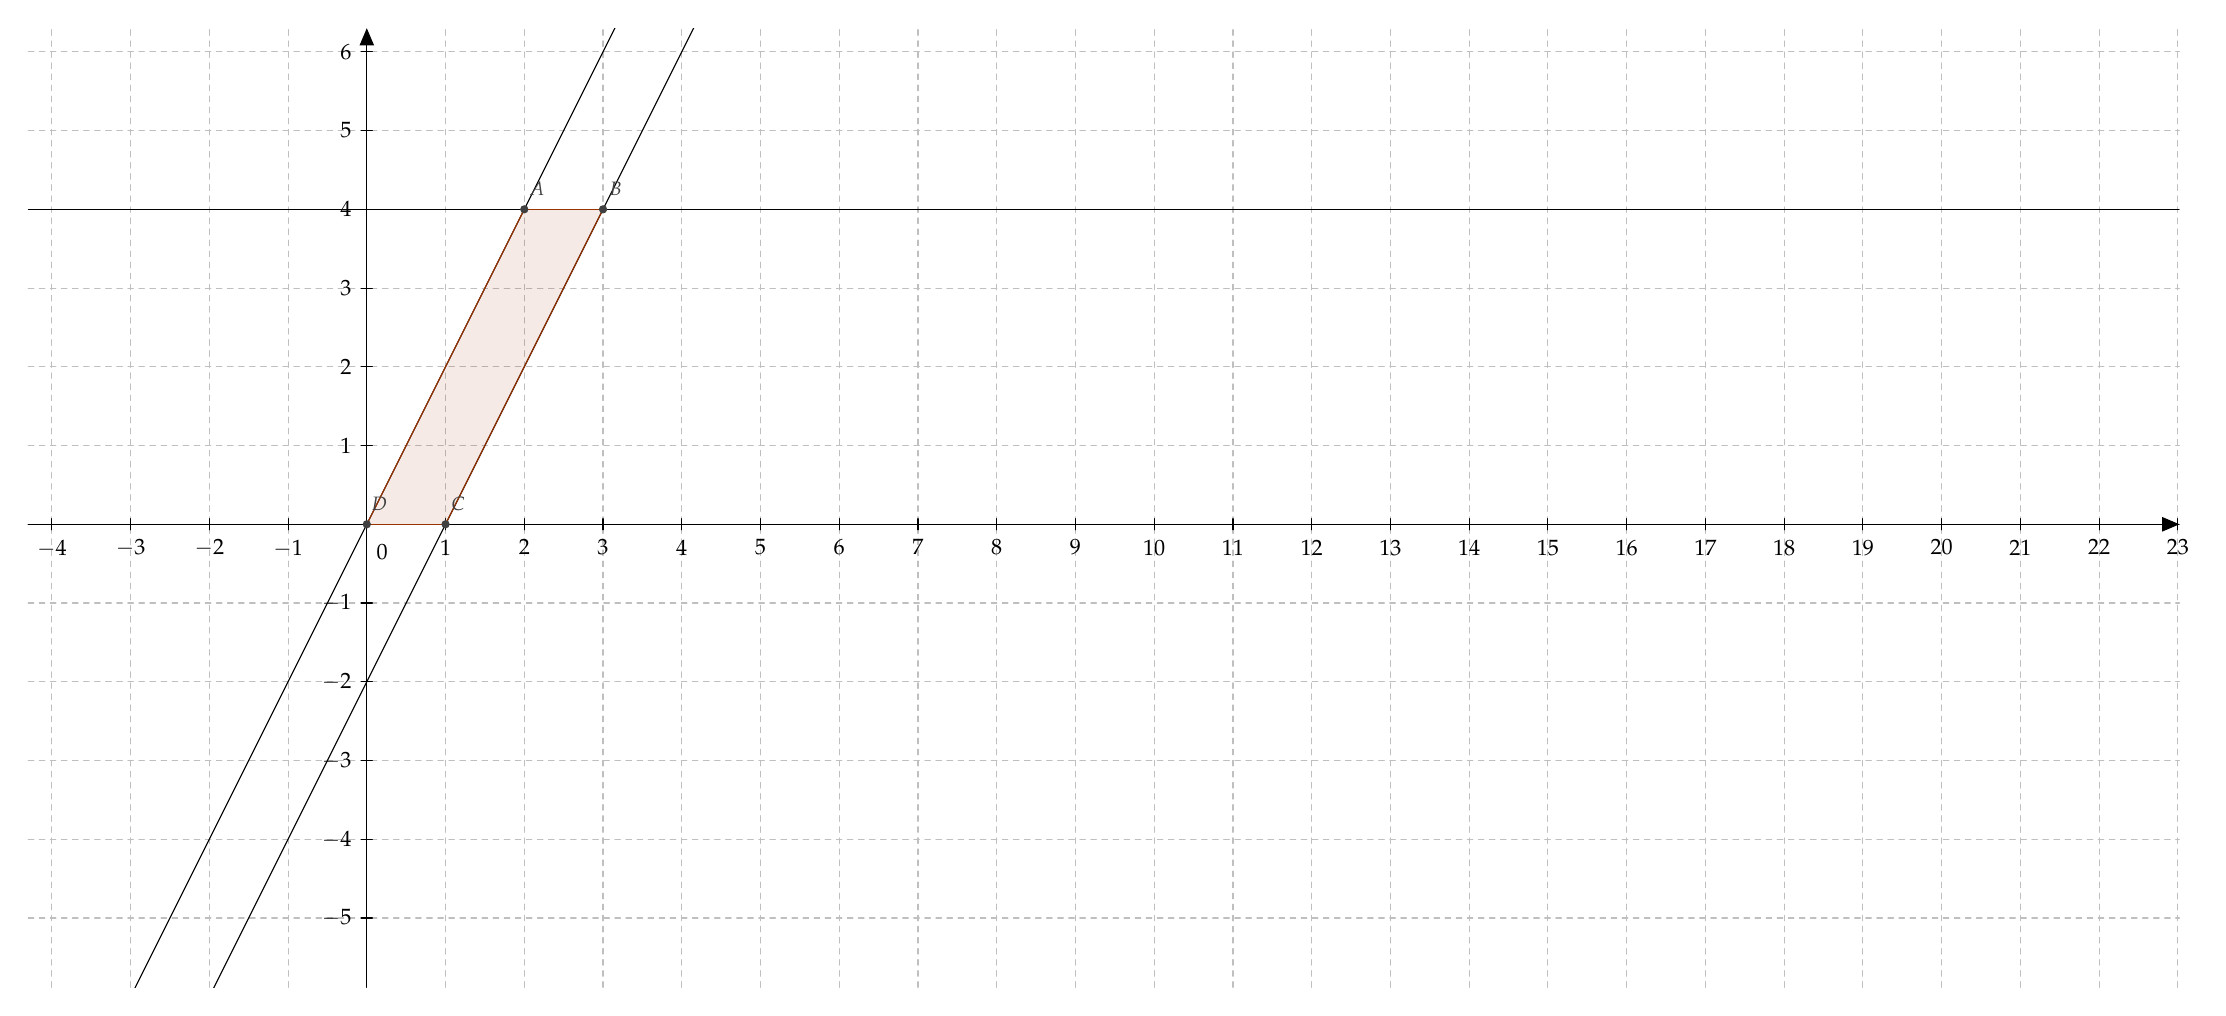
\begin{tikzpicture}[line cap=round,line join=round,>=triangle 45,x=1.0cm,y=1.0cm]
\draw [color=cqcqcq,dash pattern=on 2pt off 2pt, xstep=1.0cm,ystep=1.0cm] (-4.3,-5.88) grid (23.02,6.3);
\draw[->,color=black] (-4.3,0) -- (23.02,0);
\foreach \x in {-4,-3,-2,-1,1,2,3,4,5,6,7,8,9,10,11,12,13,14,15,16,17,18,19,20,21,22,23}
\draw[shift={(\x,0)},color=black] (0pt,2pt) -- (0pt,-2pt) node[below] {\footnotesize $\x$};
\draw[->,color=black] (0,-5.88) -- (0,6.3);
\foreach \y in {-5,-4,-3,-2,-1,1,2,3,4,5,6}
\draw[shift={(0,\y)},color=black] (2pt,0pt) -- (-2pt,0pt) node[left] {\footnotesize $\y$};
\draw[color=black] (0pt,-10pt) node[right] {\footnotesize $0$};
\clip(-4.3,-5.88) rectangle (23.02,6.3);
\fill[color=zzttqq,fill=zzttqq,fill opacity=0.1] (2,4) -- (3,4) -- (1,0) -- (0,0) -- cycle;
\draw [domain=-4.3:23.02] plot(\x,{(-0-0*\x)/1});
\draw [domain=-4.3:23.02] plot(\x,{(--4-0*\x)/1});
\draw [domain=-4.3:23.02] plot(\x,{(-0--2*\x)/1});
\draw [domain=-4.3:23.02] plot(\x,{(-2--2*\x)/1});
\draw [color=zzttqq] (2,4)-- (3,4);
\draw [color=zzttqq] (3,4)-- (1,0);
\draw [color=zzttqq] (1,0)-- (0,0);
\draw [color=zzttqq] (0,0)-- (2,4);
\begin{scriptsize}
\fill [color=uququq] (2,4) circle (1.5pt);
\draw[color=uququq] (2.16,4.26) node {$A$};
\fill [color=uququq] (3,4) circle (1.5pt);
\draw[color=uququq] (3.16,4.26) node {$B$};
\fill [color=uququq] (1,0) circle (1.5pt);
\draw[color=uququq] (1.16,0.26) node {$C$};
\fill [color=uququq] (0,0) circle (1.5pt);
\draw[color=uququq] (0.16,0.26) node {$D$};
\end{scriptsize}
\end{tikzpicture}
该区域在矩阵
$$
\begin{pmatrix}
  1&\frac{-1}{2}\\
0&\frac{1}{2}\\
\end{pmatrix}
$$
的作用下变成如下区域:\\
\begin{tikzpicture}[line cap=round,line join=round,>=triangle 45,x=1.0cm,y=1.0cm]
\draw [color=cqcqcq,dash pattern=on 1pt off 1pt, xstep=1.0cm,ystep=1.0cm] (-3.25,-2.16) grid (11.74,4.52);
\draw[->,color=black] (-3.25,0) -- (11.74,0);
\foreach \x in {-3,-2,-1,1,2,3,4,5,6,7,8,9,10,11}
\draw[shift={(\x,0)},color=black] (0pt,2pt) -- (0pt,-2pt) node[below] {\footnotesize $\x$};
\draw[->,color=black] (0,-2.16) -- (0,4.52);
\foreach \y in {-2,-1,1,2,3,4}
\draw[shift={(0,\y)},color=black] (2pt,0pt) -- (-2pt,0pt) node[left] {\footnotesize $\y$};
\draw[color=black] (0pt,-10pt) node[right] {\footnotesize $0$};
\clip(-3.25,-2.16) rectangle (11.74,4.52);
\fill[color=zzttqq,fill=zzttqq,fill opacity=0.1] (0,0) -- (0,2) -- (1,2) -- (1,0) -- cycle;
\draw [color=zzttqq] (0,0)-- (0,2);
\draw [color=zzttqq] (0,2)-- (1,2);
\draw [color=zzttqq] (1,2)-- (1,0);
\draw [color=zzttqq] (1,0)-- (0,0);
\begin{scriptsize}
\fill [color=uququq] (0,0) circle (1.5pt);
\draw[color=uququq] (0.08,0.14) node {$D$};
\fill [color=qqqqff] (1,2) circle (1.5pt);
\draw[color=qqqqff] (1.08,2.14) node {$B$};
\fill [color=xdxdff] (0,2) circle (1.5pt);
\draw[color=xdxdff] (0.08,2.14) node {$A$};
\fill [color=xdxdff] (1,0) circle (1.5pt);
\draw[color=xdxdff] (1.08,0.14) node {$C$};
\end{scriptsize}
\end{tikzpicture}
易得
$$
\int_0^4\int_{\frac{y}{2}}^{(y/2)+1}\frac{2x-y}{2}dxdy=\int_0^4\int_{v}^{v+1}udxdy=\int_0^2\int_{0}^{1}2ududv=2.
$$
\end{proof}
% ----------------------------------------------------------------------------------------
%	BIBLIOGRAPHY
% ----------------------------------------------------------------------------------------
  
\bibliographystyle{unsrt}
  
\bibliography{sample}
  
% ----------------------------------------------------------------------------------------
\end{CJK}
\end{document}